\documentclass[tikz, border=2mm]{standalone}
\usetikzlibrary{shapes, arrows.meta}

\begin{document}

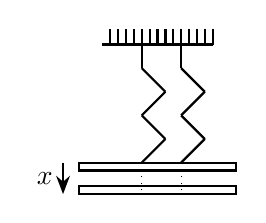
\begin{tikzpicture}[thick]
    % Support rod (horizontal)
    \draw (0.8,2) -- (2.2,2); % Shortened the support system
    
    % First Rectangle
    \draw (0.5,0.4) rectangle (2.5,0.5); % Centered the first rectangle
    
    % First Spring (tight rod)
    \draw (1.3,0.5) -- (1.6,0.8);
    \draw (1.6,0.8) -- (1.3,1.1);
    \draw (1.3,1.1) -- (1.6,1.4);
    \draw (1.6,1.4) -- (1.3,1.7);
    \draw (1.3,1.7) -- (1.3,2);
    
    % Second Rectangle (dotted)
    \draw (0.5,0.1) rectangle (2.5,0.2);
    
    % Second Spring (tight rod)
    \draw (1.8,0.5) -- (2.1,0.8);
    \draw (2.1,0.8) -- (1.8,1.1);
    \draw (1.8,1.1) -- (2.1,1.4);
    \draw (2.1,1.4) -- (1.8,1.7);
    \draw (1.8,1.7) -- (1.8,2);
    
    \foreach \i in {1,...,14}
        \draw ({0.8 + 0.1*\i},2) -- ({0.8 + 0.1*\i},2.2);
    
    \draw[thin, dotted] (1.3,0.5) -- (1.3,0.1);
    \draw[thin, dotted] (1.8,0.5) -- (1.8,0.1);
    
    % Arrow downwards for \delta x
    \draw[->, >=Stealth] (0.3, 0.5) -- node[midway, left] {\(x\)} (0.3, 0.1);
\end{tikzpicture}

\end{document}

